% Options for packages loaded elsewhere
\PassOptionsToPackage{unicode}{hyperref}
\PassOptionsToPackage{hyphens}{url}
\PassOptionsToPackage{dvipsnames,svgnames,x11names}{xcolor}
%
\documentclass[
  letterpaper,
  DIV=11,
  numbers=noendperiod]{scrartcl}

\usepackage{amsmath,amssymb}
\usepackage{iftex}
\ifPDFTeX
  \usepackage[T1]{fontenc}
  \usepackage[utf8]{inputenc}
  \usepackage{textcomp} % provide euro and other symbols
\else % if luatex or xetex
  \usepackage{unicode-math}
  \defaultfontfeatures{Scale=MatchLowercase}
  \defaultfontfeatures[\rmfamily]{Ligatures=TeX,Scale=1}
\fi
\usepackage{lmodern}
\ifPDFTeX\else  
    % xetex/luatex font selection
\fi
% Use upquote if available, for straight quotes in verbatim environments
\IfFileExists{upquote.sty}{\usepackage{upquote}}{}
\IfFileExists{microtype.sty}{% use microtype if available
  \usepackage[]{microtype}
  \UseMicrotypeSet[protrusion]{basicmath} % disable protrusion for tt fonts
}{}
\makeatletter
\@ifundefined{KOMAClassName}{% if non-KOMA class
  \IfFileExists{parskip.sty}{%
    \usepackage{parskip}
  }{% else
    \setlength{\parindent}{0pt}
    \setlength{\parskip}{6pt plus 2pt minus 1pt}}
}{% if KOMA class
  \KOMAoptions{parskip=half}}
\makeatother
\usepackage{xcolor}
\setlength{\emergencystretch}{3em} % prevent overfull lines
\setcounter{secnumdepth}{-\maxdimen} % remove section numbering
% Make \paragraph and \subparagraph free-standing
\makeatletter
\ifx\paragraph\undefined\else
  \let\oldparagraph\paragraph
  \renewcommand{\paragraph}{
    \@ifstar
      \xxxParagraphStar
      \xxxParagraphNoStar
  }
  \newcommand{\xxxParagraphStar}[1]{\oldparagraph*{#1}\mbox{}}
  \newcommand{\xxxParagraphNoStar}[1]{\oldparagraph{#1}\mbox{}}
\fi
\ifx\subparagraph\undefined\else
  \let\oldsubparagraph\subparagraph
  \renewcommand{\subparagraph}{
    \@ifstar
      \xxxSubParagraphStar
      \xxxSubParagraphNoStar
  }
  \newcommand{\xxxSubParagraphStar}[1]{\oldsubparagraph*{#1}\mbox{}}
  \newcommand{\xxxSubParagraphNoStar}[1]{\oldsubparagraph{#1}\mbox{}}
\fi
\makeatother


\providecommand{\tightlist}{%
  \setlength{\itemsep}{0pt}\setlength{\parskip}{0pt}}\usepackage{longtable,booktabs,array}
\usepackage{calc} % for calculating minipage widths
% Correct order of tables after \paragraph or \subparagraph
\usepackage{etoolbox}
\makeatletter
\patchcmd\longtable{\par}{\if@noskipsec\mbox{}\fi\par}{}{}
\makeatother
% Allow footnotes in longtable head/foot
\IfFileExists{footnotehyper.sty}{\usepackage{footnotehyper}}{\usepackage{footnote}}
\makesavenoteenv{longtable}
\usepackage{graphicx}
\makeatletter
\def\maxwidth{\ifdim\Gin@nat@width>\linewidth\linewidth\else\Gin@nat@width\fi}
\def\maxheight{\ifdim\Gin@nat@height>\textheight\textheight\else\Gin@nat@height\fi}
\makeatother
% Scale images if necessary, so that they will not overflow the page
% margins by default, and it is still possible to overwrite the defaults
% using explicit options in \includegraphics[width, height, ...]{}
\setkeys{Gin}{width=\maxwidth,height=\maxheight,keepaspectratio}
% Set default figure placement to htbp
\makeatletter
\def\fps@figure{htbp}
\makeatother

\KOMAoption{captions}{tableheading}
\makeatletter
\@ifpackageloaded{caption}{}{\usepackage{caption}}
\AtBeginDocument{%
\ifdefined\contentsname
  \renewcommand*\contentsname{Table of contents}
\else
  \newcommand\contentsname{Table of contents}
\fi
\ifdefined\listfigurename
  \renewcommand*\listfigurename{List of Figures}
\else
  \newcommand\listfigurename{List of Figures}
\fi
\ifdefined\listtablename
  \renewcommand*\listtablename{List of Tables}
\else
  \newcommand\listtablename{List of Tables}
\fi
\ifdefined\figurename
  \renewcommand*\figurename{Figure}
\else
  \newcommand\figurename{Figure}
\fi
\ifdefined\tablename
  \renewcommand*\tablename{Table}
\else
  \newcommand\tablename{Table}
\fi
}
\@ifpackageloaded{float}{}{\usepackage{float}}
\floatstyle{ruled}
\@ifundefined{c@chapter}{\newfloat{codelisting}{h}{lop}}{\newfloat{codelisting}{h}{lop}[chapter]}
\floatname{codelisting}{Listing}
\newcommand*\listoflistings{\listof{codelisting}{List of Listings}}
\makeatother
\makeatletter
\makeatother
\makeatletter
\@ifpackageloaded{caption}{}{\usepackage{caption}}
\@ifpackageloaded{subcaption}{}{\usepackage{subcaption}}
\makeatother

\ifLuaTeX
  \usepackage{selnolig}  % disable illegal ligatures
\fi
\usepackage{bookmark}

\IfFileExists{xurl.sty}{\usepackage{xurl}}{} % add URL line breaks if available
\urlstyle{same} % disable monospaced font for URLs
\hypersetup{
  pdftitle={Exploración más profunda del tema: Customer Churn Prediction},
  pdfauthor={Gerardo Montero, César Salazar, Oscar Espinoza, Andy Peralta},
  colorlinks=true,
  linkcolor={blue},
  filecolor={Maroon},
  citecolor={Blue},
  urlcolor={Blue},
  pdfcreator={LaTeX via pandoc}}


\title{Exploración más profunda del tema: Customer Churn Prediction}
\author{Gerardo Montero, César Salazar, Oscar Espinoza, Andy Peralta}
\date{2025-06-07}

\begin{document}
\maketitle


\subsection{Introducción}\label{introducciuxf3n}

En el entorno competitivo de la industria de las telecomunicaciones, la
retención de clientes se ha convertido en un desafío estratégico de
primer orden. La capacidad para predecir cuándo un cliente podría
abandonar un servicio ---lo que se conoce como \emph{customer churn}---
representa una ventaja significativa en términos de optimización de
campañas de retención, reducción de pérdidas económicas y
fortalecimiento del valor de marca.

En este contexto, el uso de modelos de predicción basados en técnicas de
\emph{Machine Learning} y \emph{Deep Learning} ha ganado una gran
relevancia en los últimos años debido a su capacidad para modelar
grandes volúmenes de datos con una alta precisión.

La presente bitácora se basa en la profundización de un estudio anterior
centrado en la predicción de abandono de clientes utilizando aprendizaje
profundo. El objetivo es investigar más a fondo la metodología empleada,
identificar las técnicas más efectivas implementadas, y comprender cómo
estas pueden ser replicadas o adaptadas para aplicaciones prácticas,
como el desarrollo de un sistema propio basado en datos de clientes de
telecomunicaciones.

El estudio de referencia es el artículo \emph{``Customer Churn
Prediction in Telecommunication Industry Using Deep Learning''} (Fujo,
Subramanian y Khder, 2022), el cual propone un enfoque robusto y
replicable que servirá de base para la implementación futura del código
y análisis del modelo.

\subsection{Exploración}\label{exploraciuxf3n}

El artículo plantea la implementación de una red neuronal profunda con
retropropagación (\emph{Deep-BP-ANN}) como alternativa más efectiva
frente a técnicas tradicionales como regresión logística, KNN, Naïve
Bayes o XGBoost.

El modelo fue entrenado y validado utilizando dos bases de datos
ampliamente reconocidas en el área: \textbf{IBM Telco} y
\textbf{Cell2Cell}, las cuales presentan escenarios reales de clientes y
problemas típicos de desbalance de clases (entre clientes que permanecen
y los que abandonan).

\subsubsection{Metodología}\label{metodologuxeda}

\begin{itemize}
\item
  \textbf{Preprocesamiento de datos:} Se aplicó imputación de valores
  faltantes, codificación de variables categóricas (label y one-hot
  encoding), y normalización de variables numéricas con varianza alta
  mediante \texttt{MinMaxScaler}.
\item
  \textbf{Selección de características:} Se usaron dos enfoques
  complementarios ---Lasso Regression y Variance Thresholding--- para
  eliminar atributos irrelevantes y mejorar la eficiencia del modelo.
\item
  \textbf{Tratamiento del desbalance:} Dada la desproporción entre
  clases (aproximadamente 26--29\% de churn en ambos conjuntos), se
  utilizó \emph{Random Oversampling}.
\item
  \textbf{Arquitectura del modelo:} El modelo Deep-BP-ANN fue optimizado
  con 250 neuronas por capa, dos capas ocultas, función de activación
  \emph{ReLU} en capas internas y \emph{sigmoid} en la capa de salida.
  También se emplearon:

  \begin{itemize}
  \tightlist
  \item
    \emph{Early Stopping}
  \item
    \emph{Activity Regularization}
  \end{itemize}
\item
  \textbf{Evaluación del modelo:} Se utilizaron validaciones
  \emph{Holdout} y \emph{10-fold Cross Validation}, y métricas como:

  \begin{itemize}
  \tightlist
  \item
    Accuracy
  \item
    Recall
  \item
    Precision
  \item
    F1-Score
  \item
    AUC
  \end{itemize}
\end{itemize}

\subsubsection{Resultados}\label{resultados}

Los resultados muestran que el modelo propuesto supera tanto a
algoritmos tradicionales como a otros modelos de deep learning:

\begin{itemize}
\tightlist
\item
  \textbf{88.12\% de exactitud} en IBM Telco (holdout)
\item
  \textbf{79.38\% de exactitud} en Cell2Cell
\end{itemize}

Esto representa mejoras respecto a modelos ANN previos (80--85\%).

\begin{quote}
La calidad y relevancia de las variables predictoras incide más que el
tamaño del dataset en el rendimiento del modelo.
\end{quote}

\subsubsection{Gráficos}\label{gruxe1ficos}

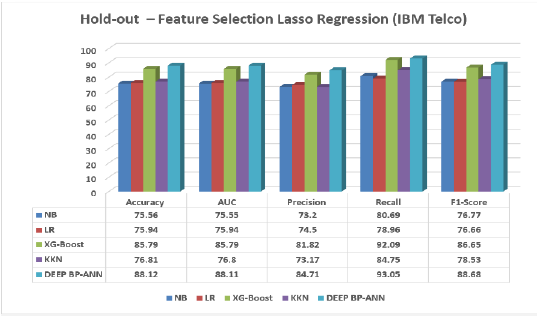
\includegraphics{imagenes/grafica_01.png}

\emph{Fuente: Fujo, Subramanian y Khder (2022)}

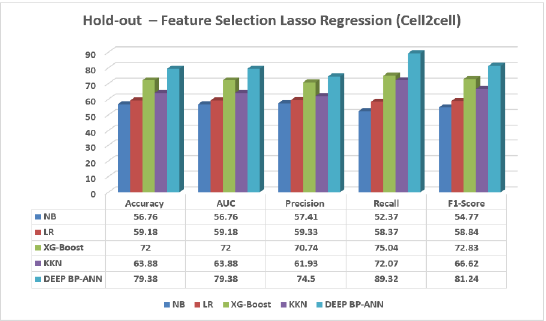
\includegraphics{imagenes/grafica_02.png}

\emph{Fuente: Fujo, Subramanian y Khder (2022)}

\subsection{Hallazgos Relevantes}\label{hallazgos-relevantes}

\begin{itemize}
\tightlist
\item
  Las variables más influyentes en IBM Telco fueron el \textbf{cargo
  total} y la \textbf{antigüedad del cliente}.
\item
  Se confirma que la calidad de las variables es más crítica que la
  cantidad de datos.
\item
  El modelo Deep-BP-ANN superó a enfoques con CNN, ANN y \emph{transfer
  learning}.
\end{itemize}

\subsection{Modelo XGB}\label{modelo-xgb}

\subsection{Modelo NB (Naive Bayes)}\label{modelo-nb-naive-bayes}

Al utilizar el modelo NB se lograron resultados bastante similares a los
del estudio, donde la presicion fue de 0.73\%, con resultados notables:
La matriz de confusión ayuda a ver si el modelo se equivoca más al
predecir que alguien no se va o que sí se va. (True Positives): 477 ---
predijo churn correctamente.

(False Positives): 539 --- dijo que se iba, pero no era cierto.

(False Negatives): 84 --- se fue, pero no lo detectó.

(True Negatives): 1010 --- predijo correctamente que no se iba.

\#Métricas de evaluación

Clase 0 (No churn): Precisión: 0.92 El modelo casi nunca se equivoca
cuando predice que el cliente no se va.

Recall: 0.65 Detecta el 65\% de los que realmente no se van.

F1-score: 0.76 Equilibrio entre precisión y recall.

Clase 1 (Churn): Precisión: 0.47 Cuando predice que se va, solo el 47\%
es cierto.

Recall: 0.85 Captura el 85\% de los clientes que efectivamente se van.

F1-score: 0.60 Moderadamente útil para detectar churn.

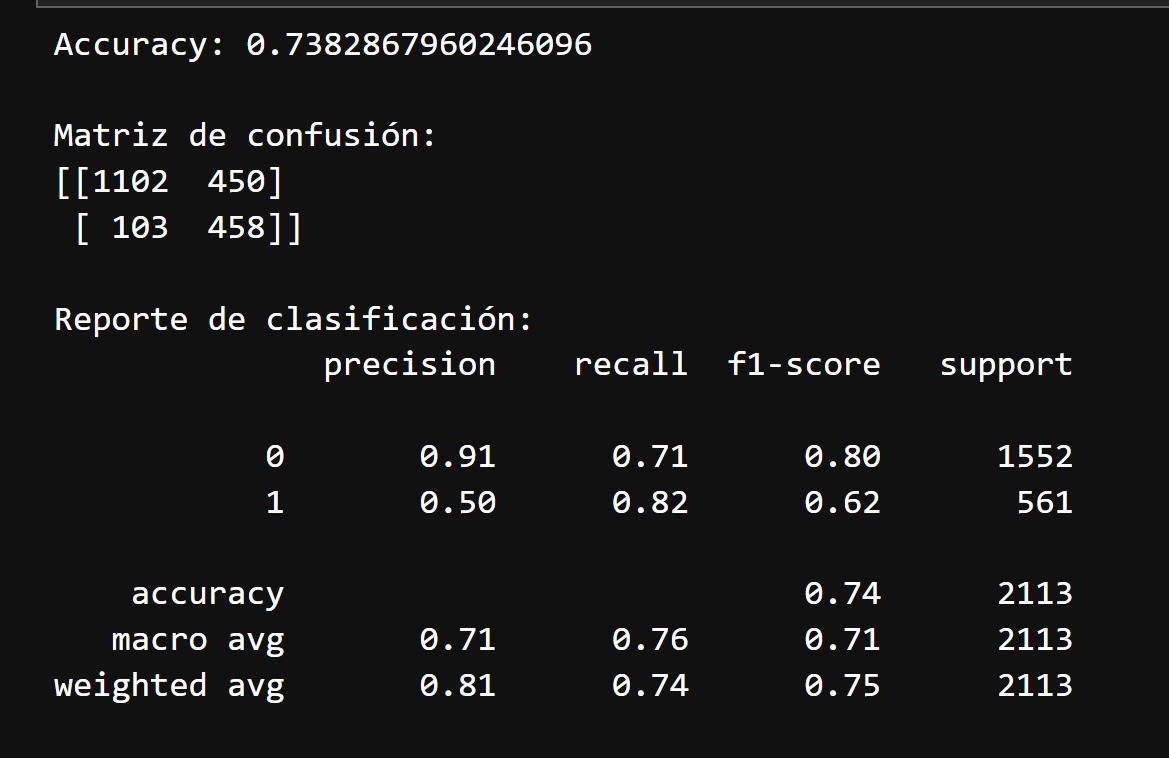
\includegraphics{imagenes/Restultados_NB_Basedatos4.png}

\subsection{Modelo BPANN}\label{modelo-bpann}

Época final (epoch): 499 El entrenamiento se detuvo en la época 499, lo
cual indica que se ejecutaron 499 ciclos completos de entrenamiento a
través de todos los datos de entrada.

Tasa de aprendizaje (learning rate): 0.300 Esta es la velocidad con la
que el modelo ajusta sus pesos en cada iteración.

Error final: 1713.518 Este valor representa el error acumulado al final
del entrenamiento.

Promedio de precisión: 79.86\%

Notamos que el uso del modelo BPANN es el mas alto, en este caso no tan
cercano al estudio debido al poder computacional que es un factor
limitande debido a el consumo energetico, de tiempo y dinero. Aun asi,
el modelo predice satisfactoriamente.

Aqui podemos ver los resultados de consola:
\includegraphics{imagenes/BPANN_resultados.png}

\subsection{Referencias}\label{referencias}

Fujo, S. W., Subramanian, S., \& Khder, M. A. (2022). \emph{Customer
churn prediction in telecommunication industry using deep learning}.
Information Sciences Letters, 11(1), 185--198.
\url{https://digitalcommons.aaru.edu.jo/isl/vol11/iss1/24}

DataCamp. (s.f.). Naive Bayes Classification with Scikit-Learn.
Recuperado el 7 de junio de 2025 de
https://www.datacamp.com/tutorial/naive-bayes-scikit-learn

Pedregosa, F., et al.~(s.f.). Naive Bayes --- scikit-learn 1.4.2
documentation. Recuperado el 7 de junio de 2025 de
https://scikit-learn.org/stable/modules/naive\_bayes.html

Enlace a repositorio GitHub:
https://github.com/CisarUli/Proyecto\_CA0305\_Grupo\_02




\end{document}
